\documentclass[conference,compsoc]{IEEEtran}
\usepackage{cite}
\usepackage{listings}
\usepackage{blindtext}
\usepackage{enumitem}
% for coding highlight
\usepackage{graphicx}
\usepackage[colorlinks=true,urlcolor=blue]{hyperref}
\usepackage{amsmath, amsthm, amssymb}
\usepackage{subfloat}
\usepackage{ulem}
\usepackage{indentfirst}
\usepackage{booktabs}
\usepackage{wrapfig,lipsum,booktabs}
\usepackage{array}
\usepackage{ulem}
\usepackage{indentfirst}
\usepackage{listings}
\usepackage{color}
\definecolor{codegreen}{rgb}{0,0.6,0}
\definecolor{codegray}{rgb}{0.5,0.5,0.5}
\definecolor{codepurple}{rgb}{0.58,0,0.82}
\definecolor{backcolour}{rgb}{0.95,0.95,0.92}


\lstdefinestyle{mystyle}{
    backgroundcolor=\color{backcolour},   
    commentstyle=\color{codegreen},
    keywordstyle=\color{magenta},
    numberstyle=\tiny\color{codegray},
    stringstyle=\color{codepurple},
    basicstyle=\footnotesize,
    breakatwhitespace=false,         
    breaklines=true,                 
    captionpos=b,                    
    keepspaces=true,                 
    numbers=left,                    
    numbersep=5pt,                  
    showspaces=false,                
    showstringspaces=false,
    showtabs=false,                  
    tabsize=2
}
\lstset{style=mystyle}

\newcommand{\subparagraph}{}
\newcolumntype{C}[1]{>{\centering\let\newline\\\arraybackslash\hspace{0pt}}m{#1}}

\begin{document}
\title{
	Deep Learning Course Proposal \\
	Passenger Screening Algorithm Challenge \\
}


% author names and affiliations
% use a multiple column layout for up to three different
% affiliations
\author{
	\IEEEauthorblockN{Yuyang Rong}
	\IEEEauthorblockA{
		School of Information Science and Technology \\
		ShanghaiTech University \\
		Student ID: 69850764 \\
	}
\and
	\IEEEauthorblockN{Peng Ding}
	\IEEEauthorblockA{
		School of Information Science and Technology \\
		ShanghaiTech University \\
		Student ID: 79406120 \\
	}
}

\maketitle

\section{Problem Description}
	\par The safety issue has always been a major concern since the day that aviation was civilized. 
	Detecting whether passengers are carrying any prohibited items is one of the key steps before passenger board the plane. 
	Conventionally, passengers are required to be screened and physically examined by Transportation Security Administration(TSA) staffs. 
	Such procedure takes time and effort to operate, without guarantee of any kind that the checking is accurate. 
	Whereas complaints call upon the invasion of personal privacy. 
	With all these being considered, people rarely consider the traditional security check as a satisfactory experience. 
	We propose a computer vision approach, utilizing deep learning method by examining critical positions of human gestures, to facilitate with the detection of prohibited items.
	\par To tackle this problem, first we have to partition human bodies into 17 parts, see Fig\ref{bodyzones}
	\begin{figure} [ht]
		\centering
		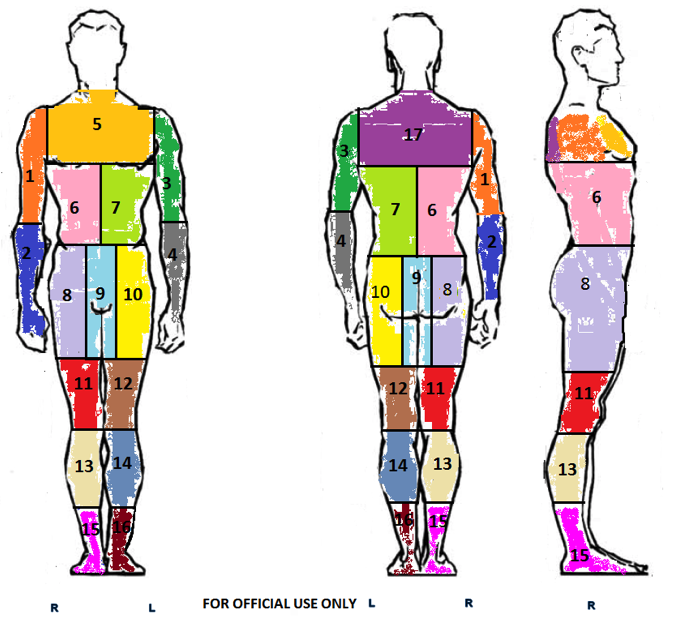
\includegraphics[width=\linewidth]{../Pic/body_zones}
		\caption{17 zones of human body.}
		\label{bodyzones}
	\end{figure}
	\subsection{A dip into labels}
		\par We have extracted all the labels from the given file \textit{stage1\_labels.csv}. We plot the following table:
		\begin{table}[h]
			\centering
			\label{labels}
			\begin{tabular}{|c|c|c|c|}
			\hline
			Zone   & Sum & Images & PerCent \\ \hline
			Zone1  & 133 & 1147  & 11.60\% \\ \hline
			Zone2  & 126 & 1147  & 10.99\% \\ \hline
			Zone8  & 124 & 1147  & 10.81\% \\ \hline
			Zone14 & 122 & 1147  & 10.64\% \\ \hline
			Zone15 & 118 & 1147  & 10.29\% \\ \hline
			Zone11 & 116 & 1147  & 10.11\% \\ \hline
			Zone6  & 116 & 1147  & 10.11\% \\ \hline
			Zone13 & 110 & 1147  & 9.59\%  \\ \hline
			Zone16 & 109 & 1147  & 9.50\%  \\ \hline
			Zone4  & 108 & 1147  & 9.42\%  \\ \hline
			Zone5  & 106 & 1147  & 9.24\%  \\ \hline
			Zone3  & 104 & 1147  & 9.07\%  \\ \hline
			Zone12 & 101 & 1147  & 8.81\%  \\ \hline
			Zone10 & 100 & 1147  & 8.72\%  \\ \hline
			Zone17 & 95  & 1147  & 8.28\%  \\ \hline
			Zone7  & 93  & 1147  & 8.11\%  \\ \hline
			Zone9  & 90  & 1147  & 7.85\%  \\ \hline
			Total  & 1871  &   & 9.595\%  \\ \hline
			\end{tabular}
			\caption{Positive label distribution.}
		\end{table}
		\begin{figure} [h]
			\centering
			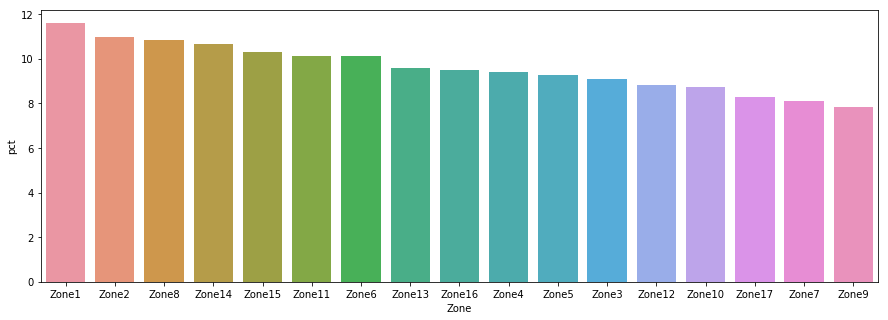
\includegraphics[width=\linewidth]{../Pic/bars}
			\caption{Visualization of the positive label distribution.}
			\label{bars}
		\end{figure}
	\subsubsection{Broken data} In total there are 1247 human scans, but only 1147 of them are labeled, besides, not everyone has all 17 zones labeled. 
	\par Besides, after seen all 16 images of one subject, the dangerous object is rather ambiguous and not clear, which made this task even harder.
	\begin{figure}[h] \label{ffefec}
		\centering
		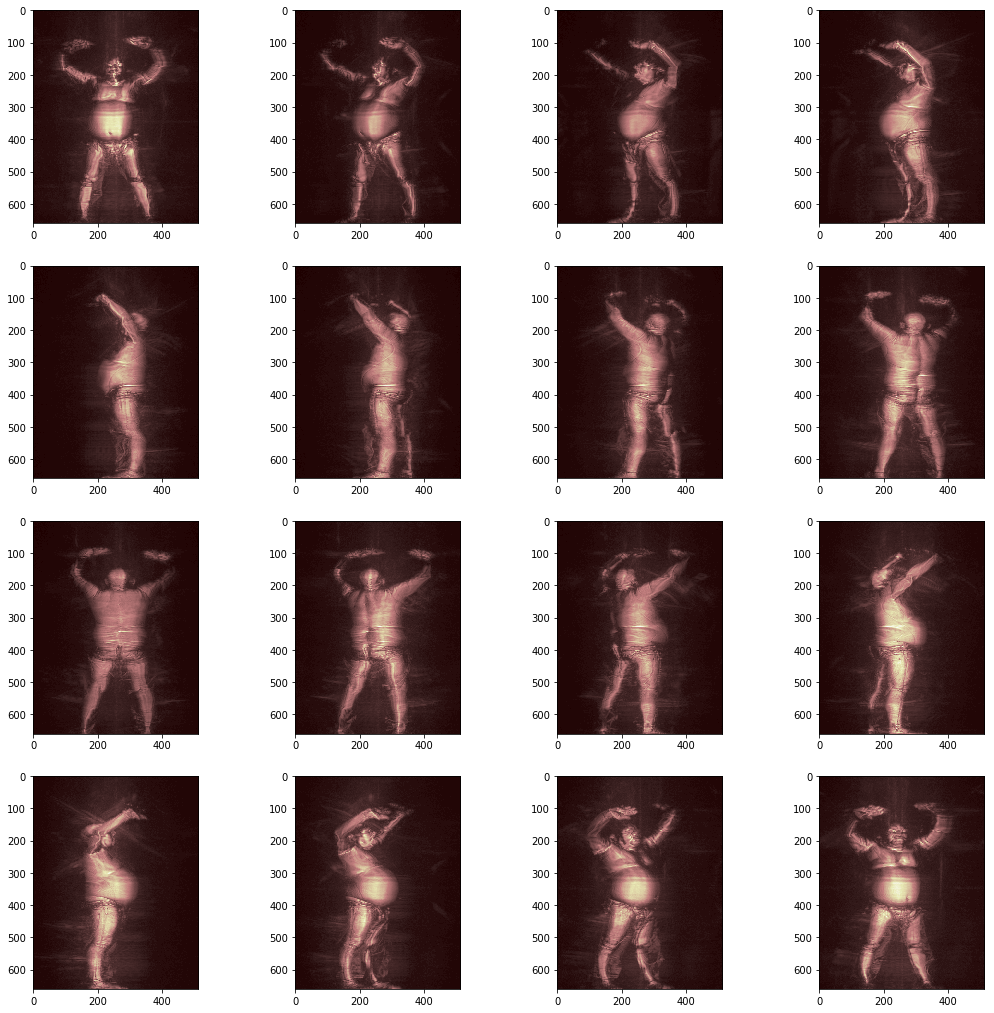
\includegraphics[width=0.9\linewidth]{../Pic/ffefec0cd4e1e2c3fe64bb93f082efdd}
		\caption{This passenger is labeled to have objects in is left arm and crotch. The back of his left arm is abnormal(dark).}
	\end{figure}
	\subsubsection{Too few positive} It is depressing to see the fact that there isn't much positive cases in data set when we know that deep networks loves positive case.	
	\subsubsection{Possibly rigged data} The most dangerous objects actually occur in right arm, this alerts us since it's hard to hide something in your right arm. What we were expecting was zone 6~10, which, in turn, had a relatively low occurrence.  
	\par We believe since these data only occurs in stage 1, there will be more common and reasonable cases in stage 2.

	\par We are given scans of one person, each scan have 22.5 degrees difference, thus in total we have 16 images per person. Each image has resolution 512*660. 
	
\section{Data Preprocessing}
	\subsection{Image Crop}
		\par We have considered the possibility of taking 512*660*16 images as input and a vector of size 17*1 describing the possibility of presence of dangerous objects. However, considering there isn't much positive outcomes, we decided to crop the images and for each zone, ask the algorithm to only see certain sector of the image.
		\par The image is cropped into 16 sectors, each sector has size 250*250 pixels. The table listed the upper left conner of each sector:
		\begin{figure}[h] \label{cropped}
			\centering
			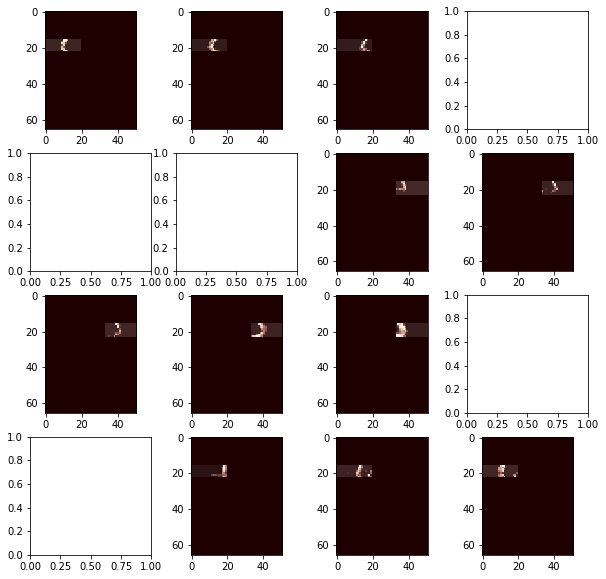
\includegraphics[width=0.9\linewidth]{../Pic/cropped}
			\caption{A cropped example of the man shown before.}
		\end{figure}
		\begin{table}[h]
			\centering
			\label{region}
			\begin{tabular}{ccc}
				\hline
				Region \# & x   & y   \\ \hline
				1         & 50  & 50  \\ \hline
				2         & 0   & 0   \\ \hline
				3         & 50  & 250 \\ \hline
				4         & 250 & 0   \\ \hline
				5         & 150 & 150 \\ \hline
				6         & 200 & 100 \\ \hline
				7         & 200 & 150 \\ \hline
				8         & 250 & 50  \\ \hline
				9         & 250 & 150 \\ \hline
				10        & 300 & 200 \\ \hline
				11        & 400 & 100 \\ \hline
				12        & 350 & 200 \\ \hline
				13        & 410 & 0   \\ \hline
				14        & 410 & 200 \\ \hline
				15        & 410 & 0   \\ \hline
				16        & 410 & 200 \\ \hline
			\end{tabular}
			\caption{Region distribution.}
		\end{table}
	\subsection{Zone assignment}
		\par Now that we have already cropped each image, we will assign each region to it's zones. This makes recognition on each zone easier. Now that no zone can be shown in all 16 images, we will represent it by a None in python.
		\par We have done the pre-calculation to assign sectors based on the index of the image. For example, threat zone 1(Right Bicep) can be see in sector 1 in image 0, 1, 2, 13, 14, 15; in sector 3 in image 6 to 10. Thus in python we write:
		\begin{lstlisting}[language = python]
zone_slice_list = [ [ # threat zone 1
   sector01_pts, sector01_pts, sector01_pts, None, None, None, sector03_pts, sector03_pts, sector03_pts, sector03_pts, sector03_pts, None, None, sector01_pts, sector01_pts, sector01_pts ],
   # threat zone 2
   # ...... 
]
		\end{lstlisting}
	\subsection{Error Canceling and Center Shift}
		\par As shown in \ref{noisy}, the scan data can be rather noisy. Our solution is to add a threshold to it. The threshold we choose is 12 in a gray scale image.
		\begin{figure}[h] \label{noisy}
			\centering
			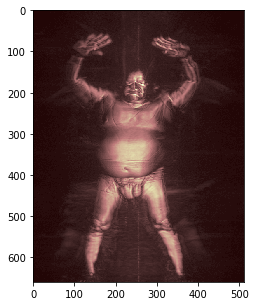
\includegraphics[width=0.7\linewidth]{../Pic/noisy}
			\caption{The scan data is rather noisy.}
		\end{figure}
		\par For each region we have cropped, we will zero-mean it and normalize it.
\section{Approach}
	\par Now that we have cropped each image and assigned them to 17 zones. We can tackle each zones once at a time. We will build a network for all zones and then train/test them separately.
	\par For each zone, we have established a deep network. Currently, we only do tests on the first zone, which is Right arm. The network architecture is the following:
	\begin{itemize}
		\item Convlution. 32 kernels with size 3x3 will be applied. 
		\item MaxPool.  2x2 pool size with stride 1.
		\item Flatten. After that we will flatten our pool and use fully connected.
		\item Dropout, with dropout rate 0.5.
		\item Fully Connected.
		\item Softmax.
	\end{itemize}
	\par This is our current design of network. We are still building this network and about to run tests on it. After that we will evaluate how does the deep learning method compete against the sparse coding method.
	\par Now we only have a rough idea of utilizing PCA. Since all the image is so aligned and the background is black, we can construct a eigen-human and reconstruct any test human. If there exists some part that have huge error, we will rule this human to have dangerous objects with him and give a rough location of the object. With a clear idea of the existence of the object and a rough position, we can use deep network afterwards.
	\par Also, the next version of our network will consist of consecutive parts -- the network for image registration, and the detection network. The first network for image registration helps to register all the view of provided date to a selected template one. We believe registration can help to reduce the spatial error caused by different human figure. But we are also concerned that such deformation could skew the shape for potential threats, therefore, an experiment will be added to assess how the registration helps with the detection. We plan to develop both the RNN version and CNN version for detection network. Since we see potential similarity between this task and image captioning, and the latter one demonstrates the advantage of RNN over other methods.
\bibliographystyle{IEEEtran}
%% De-comment this line if you have any reference.
%% And don't forget to change .bib file.
% \bibliography{milestone}
\end{document}
